\documentclass[1p]{elsarticle_modified}
%\bibliographystyle{elsarticle-num}

%\usepackage[colorlinks]{hyperref}
%\usepackage{abbrmath_seonhwa} %\Abb, \Ascr, \Acal ,\Abf, \Afrak
\usepackage{amsfonts}
\usepackage{amssymb}
\usepackage{amsmath}
\usepackage{amsthm}
\usepackage{scalefnt}
\usepackage{amsbsy}
\usepackage{kotex}
\usepackage{caption}
\usepackage{subfig}
\usepackage{color}
\usepackage{graphicx}
\usepackage{xcolor} %% white, black, red, green, blue, cyan, magenta, yellow
\usepackage{float}
\usepackage{setspace}
\usepackage{hyperref}

\usepackage{tikz}
\usetikzlibrary{arrows}

\usepackage{multirow}
\usepackage{array} % fixed length table
\usepackage{hhline}

%%%%%%%%%%%%%%%%%%%%%
\makeatletter
\renewcommand*\env@matrix[1][\arraystretch]{%
	\edef\arraystretch{#1}%
	\hskip -\arraycolsep
	\let\@ifnextchar\new@ifnextchar
	\array{*\c@MaxMatrixCols c}}
\makeatother %https://tex.stackexchange.com/questions/14071/how-can-i-increase-the-line-spacing-in-a-matrix
%%%%%%%%%%%%%%%

\usepackage[normalem]{ulem}

\newcommand{\msout}[1]{\ifmmode\text{\sout{\ensuremath{#1}}}\else\sout{#1}\fi}
%SOURCE: \msout is \stkout macro in https://tex.stackexchange.com/questions/20609/strikeout-in-math-mode

\newcommand{\cancel}[1]{
	\ifmmode
	{\color{red}\msout{#1}}
	\else
	{\color{red}\sout{#1}}
	\fi
}

\newcommand{\add}[1]{
	{\color{blue}\uwave{#1}}
}

\newcommand{\replace}[2]{
	\ifmmode
	{\color{red}\msout{#1}}{\color{blue}\uwave{#2}}
	\else
	{\color{red}\sout{#1}}{\color{blue}\uwave{#2}}
	\fi
}

\newcommand{\Sol}{\mathcal{S}} %segment
\newcommand{\D}{D} %diagram
\newcommand{\A}{\mathcal{A}} %arc


%%%%%%%%%%%%%%%%%%%%%%%%%%%%%5 test

\def\sl{\operatorname{\textup{SL}}(2,\Cbb)}
\def\psl{\operatorname{\textup{PSL}}(2,\Cbb)}
\def\quan{\mkern 1mu \triangleright \mkern 1mu}

\theoremstyle{definition}
\newtheorem{thm}{Theorem}[section]
\newtheorem{prop}[thm]{Proposition}
\newtheorem{lem}[thm]{Lemma}
\newtheorem{ques}[thm]{Question}
\newtheorem{cor}[thm]{Corollary}
\newtheorem{defn}[thm]{Definition}
\newtheorem{exam}[thm]{Example}
\newtheorem{rmk}[thm]{Remark}
\newtheorem{alg}[thm]{Algorithm}

\newcommand{\I}{\sqrt{-1}}
\begin{document}

%\begin{frontmatter}
%
%\title{Boundary parabolic representations of knots up to 8 crossings}
%
%%% Group authors per affiliation:
%\author{Yunhi Cho} 
%\address{Department of Mathematics, University of Seoul, Seoul, Korea}
%\ead{yhcho@uos.ac.kr}
%
%
%\author{Seonhwa Kim} %\fnref{s_kim}}
%\address{Center for Geometry and Physics, Institute for Basic Science, Pohang, 37673, Korea}
%\ead{ryeona17@ibs.re.kr}
%
%\author{Hyuk Kim}
%\address{Department of Mathematical Sciences, Seoul National University, Seoul 08826, Korea}
%\ead{hyukkim@snu.ac.kr}
%
%\author{Seokbeom Yoon}
%\address{Department of Mathematical Sciences, Seoul National University, Seoul, 08826,  Korea}
%\ead{sbyoon15@snu.ac.kr}
%
%\begin{abstract}
%We find all boundary parabolic representation of knots up to 8 crossings.
%
%\end{abstract}
%\begin{keyword}
%    \MSC[2010] 57M25 
%\end{keyword}
%
%\end{frontmatter}

%\linenumbers
%\tableofcontents
%
\newcommand\colored[1]{\textcolor{white}{\rule[-0.35ex]{0.8em}{1.4ex}}\kern-0.8em\color{red} #1}%
%\newcommand\colored[1]{\textcolor{white}{ #1}\kern-2.17ex	\textcolor{white}{ #1}\kern-1.81ex	\textcolor{white}{ #1}\kern-2.15ex\color{red}#1	}

{\Large $\underline{12n_{0197}~(K12n_{0197})}$}

\setlength{\tabcolsep}{10pt}
\renewcommand{\arraystretch}{1.6}
\vspace{1cm}\begin{tabular}{m{100pt}>{\centering\arraybackslash}m{274pt}}
\multirow{5}{120pt}{
	\centering
	\includegraphics[width=112pt]{../../../GIT/diagram.site/Diagrams/png/2286_12n_0197.png}\\
\ \ \ A knot diagram\footnotemark}&
\allowdisplaybreaks
\textbf{Linearized knot diagam} \\
\cline{2-2}
 &
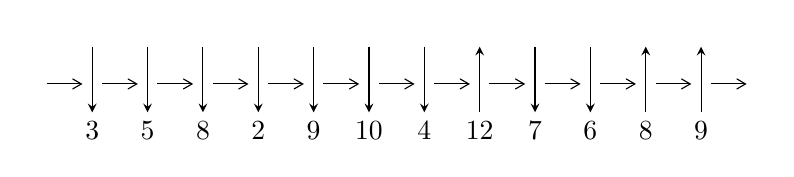
\begin{tikzpicture}[x=20pt, y=17pt]
	% nodes
	\node (C0) at (0, 0) {};
	\node (C1) at (1, 0) {};
	\node (C1U) at (1, +1) {};
	\node (C1D) at (1, -1) {3};

	\node (C2) at (2, 0) {};
	\node (C2U) at (2, +1) {};
	\node (C2D) at (2, -1) {5};

	\node (C3) at (3, 0) {};
	\node (C3U) at (3, +1) {};
	\node (C3D) at (3, -1) {8};

	\node (C4) at (4, 0) {};
	\node (C4U) at (4, +1) {};
	\node (C4D) at (4, -1) {2};

	\node (C5) at (5, 0) {};
	\node (C5U) at (5, +1) {};
	\node (C5D) at (5, -1) {9};

	\node (C6) at (6, 0) {};
	\node (C6U) at (6, +1) {};
	\node (C6D) at (6, -1) {10};

	\node (C7) at (7, 0) {};
	\node (C7U) at (7, +1) {};
	\node (C7D) at (7, -1) {4};

	\node (C8) at (8, 0) {};
	\node (C8U) at (8, +1) {};
	\node (C8D) at (8, -1) {12};

	\node (C9) at (9, 0) {};
	\node (C9U) at (9, +1) {};
	\node (C9D) at (9, -1) {7};

	\node (C10) at (10, 0) {};
	\node (C10U) at (10, +1) {};
	\node (C10D) at (10, -1) {6};

	\node (C11) at (11, 0) {};
	\node (C11U) at (11, +1) {};
	\node (C11D) at (11, -1) {8};

	\node (C12) at (12, 0) {};
	\node (C12U) at (12, +1) {};
	\node (C12D) at (12, -1) {9};
	\node (C13) at (13, 0) {};

	% arrows
	\draw[->,>={angle 60}]
	(C0) edge (C1) (C1) edge (C2) (C2) edge (C3) (C3) edge (C4) (C4) edge (C5) (C5) edge (C6) (C6) edge (C7) (C7) edge (C8) (C8) edge (C9) (C9) edge (C10) (C10) edge (C11) (C11) edge (C12) (C12) edge (C13) ;	\draw[->,>=stealth]
	(C1U) edge (C1D) (C2U) edge (C2D) (C3U) edge (C3D) (C4U) edge (C4D) (C5U) edge (C5D) (C6U) edge (C6D) (C7U) edge (C7D) (C8D) edge (C8U) (C9U) edge (C9D) (C10U) edge (C10D) (C11D) edge (C11U) (C12D) edge (C12U) ;
	\end{tikzpicture} \\
\hhline{~~} \\& 
\textbf{Solving Sequence} \\ \cline{2-2} 
 &
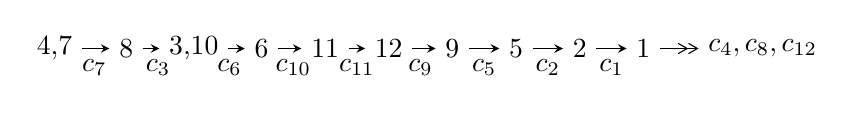
\begin{tikzpicture}[x=23pt, y=7pt]
	% node
	\node (A0) at (-1/8, 0) {4,7};
	\node (A1) at (1, 0) {8};
	\node (A2) at (33/16, 0) {3,10};
	\node (A3) at (25/8, 0) {6};
	\node (A4) at (33/8, 0) {11};
	\node (A5) at (41/8, 0) {12};
	\node (A6) at (49/8, 0) {9};
	\node (A7) at (57/8, 0) {5};
	\node (A8) at (65/8, 0) {2};
	\node (A9) at (73/8, 0) {1};
	\node (C1) at (1/2, -1) {$c_{7}$};
	\node (C2) at (3/2, -1) {$c_{3}$};
	\node (C3) at (21/8, -1) {$c_{6}$};
	\node (C4) at (29/8, -1) {$c_{10}$};
	\node (C5) at (37/8, -1) {$c_{11}$};
	\node (C6) at (45/8, -1) {$c_{9}$};
	\node (C7) at (53/8, -1) {$c_{5}$};
	\node (C8) at (61/8, -1) {$c_{2}$};
	\node (C9) at (69/8, -1) {$c_{1}$};
	\node (A10) at (11, 0) {$c_{4},c_{8},c_{12}$};

	% edge
	\draw[->,>=stealth]	
	(A0) edge (A1) (A1) edge (A2) (A2) edge (A3) (A3) edge (A4) (A4) edge (A5) (A5) edge (A6) (A6) edge (A7) (A7) edge (A8) (A8) edge (A9) ;
	\draw[->>,>={angle 60}]	
	(A9) edge (A10);
\end{tikzpicture} \\ 

\end{tabular} \\

\footnotetext{
The image of knot diagram is generated by the software ``\textbf{Draw programme}" developed by Andrew Bartholomew(\url{http://www.layer8.co.uk/maths/draw/index.htm\#Running-draw}), where we modified some parts for our purpose(\url{https://github.com/CATsTAILs/LinksPainter}).
}\phantom \\ \newline 
\centering \textbf{Ideals for irreducible components\footnotemark of $X_{\text{par}}$} 
 
\begin{align*}
I^u_{1}&=\langle 
-8.18355\times10^{119} u^{63}-1.02834\times10^{120} u^{62}+\cdots+6.77073\times10^{121} b-4.36658\times10^{121},\\
\phantom{I^u_{1}}&\phantom{= \langle  }1.74383\times10^{121} u^{63}+1.62828\times10^{121} u^{62}+\cdots+6.09366\times10^{122} a-5.03534\times10^{122},\\
\phantom{I^u_{1}}&\phantom{= \langle  }u^{64}+2 u^{63}+\cdots-36 u-36\rangle \\
I^u_{2}&=\langle 
-3 u^2 a+a u+3 u^2+5 b-2 a- u+7,\;-4 u^2 a+a^2+2 a u+7 u^2-6 a-2 u+17,\;u^3- u^2+2 u-1\rangle \\
I^u_{3}&=\langle 
b,\;-2 u^2+a- u-3,\;u^3+u^2+2 u+1\rangle \\
\\
I^v_{1}&=\langle 
a,\;b-3 v+1,\;3 v^2-3 v+1\rangle \\
\end{align*}
\raggedright * 4 irreducible components of $\dim_{\mathbb{C}}=0$, with total 75 representations.\\
\footnotetext{All coefficients of polynomials are rational numbers. But the coefficients are sometimes approximated in decimal forms when there is not enough margin.}
\newpage
\renewcommand{\arraystretch}{1}
\centering \section*{I. $I^u_{1}= \langle -8.18\times10^{119} u^{63}-1.03\times10^{120} u^{62}+\cdots+6.77\times10^{121} b-4.37\times10^{121},\;1.74\times10^{121} u^{63}+1.63\times10^{121} u^{62}+\cdots+6.09\times10^{122} a-5.04\times10^{122},\;u^{64}+2 u^{63}+\cdots-36 u-36 \rangle$}
\flushleft \textbf{(i) Arc colorings}\\
\begin{tabular}{m{7pt} m{180pt} m{7pt} m{180pt} }
\flushright $a_{4}=$&$\begin{pmatrix}0\\u\end{pmatrix}$ \\
\flushright $a_{7}=$&$\begin{pmatrix}1\\0\end{pmatrix}$ \\
\flushright $a_{8}=$&$\begin{pmatrix}1\\u^2\end{pmatrix}$ \\
\flushright $a_{3}=$&$\begin{pmatrix}u\\u^3+u\end{pmatrix}$ \\
\flushright $a_{10}=$&$\begin{pmatrix}-0.0286172 u^{63}-0.0267209 u^{62}+\cdots+6.11396 u+0.826324\\0.0120867 u^{63}+0.0151881 u^{62}+\cdots-2.44925 u+0.644920\end{pmatrix}$ \\
\flushright $a_{6}=$&$\begin{pmatrix}-0.00662501 u^{63}+0.00268962 u^{62}+\cdots+0.595026 u-0.834195\\-0.00664903 u^{63}-0.0289554 u^{62}+\cdots+1.40621 u+1.36782\end{pmatrix}$ \\
\flushright $a_{11}=$&$\begin{pmatrix}-0.0183635 u^{63}-0.0249695 u^{62}+\cdots+5.48546 u-0.126144\\0.00140169 u^{63}+0.0235025 u^{62}+\cdots-1.73632 u-1.16399\end{pmatrix}$ \\
\flushright $a_{12}=$&$\begin{pmatrix}-0.0101569 u^{63}+0.00172136 u^{62}+\cdots+3.98696 u-1.71340\\-0.00147268 u^{63}+0.0111679 u^{62}+\cdots-1.07088 u-0.793992\end{pmatrix}$ \\
\flushright $a_{9}=$&$\begin{pmatrix}-0.0165305 u^{63}-0.0115329 u^{62}+\cdots+3.66471 u+1.47124\\0.0120867 u^{63}+0.0151881 u^{62}+\cdots-2.44925 u+0.644920\end{pmatrix}$ \\
\flushright $a_{5}=$&$\begin{pmatrix}-0.00128622 u^{63}-0.00466939 u^{62}+\cdots+2.09437 u-0.413947\\-0.000693282 u^{63}-0.0414084 u^{62}+\cdots+0.539582 u+3.47925\end{pmatrix}$ \\
\flushright $a_{2}=$&$\begin{pmatrix}0.00597049 u^{63}-0.0314814 u^{62}+\cdots-1.43299 u+3.96869\\0.0313178 u^{63}+0.0159753 u^{62}+\cdots-0.686893 u+1.99154\end{pmatrix}$ \\
\flushright $a_{1}=$&$\begin{pmatrix}0.000592942 u^{63}-0.0367390 u^{62}+\cdots-1.55479 u+3.89320\\0.0243989 u^{63}+0.00752519 u^{62}+\cdots-0.804368 u+2.11396\end{pmatrix}$\\&\end{tabular}
\flushleft \textbf{(ii) Obstruction class $= -1$}\\~\\
\flushleft \textbf{(iii) Cusp Shapes $= 0.144774 u^{63}+0.289389 u^{62}+\cdots-34.9857 u-14.7964$}\\~\\
\newpage\renewcommand{\arraystretch}{1}
\flushleft \textbf{(iv) u-Polynomials at the component}\newline \\
\begin{tabular}{m{50pt}|m{274pt}}
Crossings & \hspace{64pt}u-Polynomials at each crossing \\
\hline $$\begin{aligned}c_{1}\end{aligned}$$&$\begin{aligned}
&u^{64}+34 u^{63}+\cdots+295 u+81
\end{aligned}$\\
\hline $$\begin{aligned}c_{2},c_{4}\end{aligned}$$&$\begin{aligned}
&u^{64}-6 u^{63}+\cdots-41 u+9
\end{aligned}$\\
\hline $$\begin{aligned}c_{3},c_{7}\end{aligned}$$&$\begin{aligned}
&u^{64}+2 u^{63}+\cdots-36 u-36
\end{aligned}$\\
\hline $$\begin{aligned}c_{5}\end{aligned}$$&$\begin{aligned}
&u^{64}+2 u^{63}+\cdots+14008 u+1448
\end{aligned}$\\
\hline $$\begin{aligned}c_{6},c_{9},c_{10}\end{aligned}$$&$\begin{aligned}
&u^{64}-2 u^{63}+\cdots-8 u+8
\end{aligned}$\\
\hline $$\begin{aligned}c_{8},c_{11},c_{12}\end{aligned}$$&$\begin{aligned}
&u^{64}-5 u^{63}+\cdots+77 u-49
\end{aligned}$\\
\hline
\end{tabular}\\~\\
\newpage\renewcommand{\arraystretch}{1}
\flushleft \textbf{(v) Riley Polynomials at the component}\newline \\
\begin{tabular}{m{50pt}|m{274pt}}
Crossings & \hspace{64pt}Riley Polynomials at each crossing \\
\hline $$\begin{aligned}c_{1}\end{aligned}$$&$\begin{aligned}
&y^{64}-2 y^{63}+\cdots-197995 y+6561
\end{aligned}$\\
\hline $$\begin{aligned}c_{2},c_{4}\end{aligned}$$&$\begin{aligned}
&y^{64}-34 y^{63}+\cdots-295 y+81
\end{aligned}$\\
\hline $$\begin{aligned}c_{3},c_{7}\end{aligned}$$&$\begin{aligned}
&y^{64}+24 y^{63}+\cdots+8136 y+1296
\end{aligned}$\\
\hline $$\begin{aligned}c_{5}\end{aligned}$$&$\begin{aligned}
&y^{64}-28 y^{63}+\cdots-37440 y+2096704
\end{aligned}$\\
\hline $$\begin{aligned}c_{6},c_{9},c_{10}\end{aligned}$$&$\begin{aligned}
&y^{64}+56 y^{63}+\cdots-2240 y+64
\end{aligned}$\\
\hline $$\begin{aligned}c_{8},c_{11},c_{12}\end{aligned}$$&$\begin{aligned}
&y^{64}-25 y^{63}+\cdots-103635 y+2401
\end{aligned}$\\
\hline
\end{tabular}\\~\\
\newpage\flushleft \textbf{(vi) Complex Volumes and Cusp Shapes}
$$\begin{array}{c|c|c}  
\text{Solutions to }I^u_{1}& \I (\text{vol} + \sqrt{-1}CS) & \text{Cusp shape}\\
 \hline 
\begin{aligned}
u &= \phantom{-}0.371724 + 0.987147 I \\
a &= \phantom{-}0.34956 - 2.12621 I \\
b &= -0.00833 + 1.56770 I\end{aligned}
 & \phantom{-}7.22646 - 4.24018 I & -1.56965 + 6.79694 I \\ \hline\begin{aligned}
u &= \phantom{-}0.371724 - 0.987147 I \\
a &= \phantom{-}0.34956 + 2.12621 I \\
b &= -0.00833 - 1.56770 I\end{aligned}
 & \phantom{-}7.22646 + 4.24018 I & -1.56965 - 6.79694 I \\ \hline\begin{aligned}
u &= -0.851897 + 0.643385 I \\
a &= \phantom{-}0.219665 + 0.339736 I \\
b &= \phantom{-}0.734413 - 0.053249 I\end{aligned}
 & -1.92756 + 0.31252 I & -6.62839 - 0.48650 I \\ \hline\begin{aligned}
u &= -0.851897 - 0.643385 I \\
a &= \phantom{-}0.219665 - 0.339736 I \\
b &= \phantom{-}0.734413 + 0.053249 I\end{aligned}
 & -1.92756 - 0.31252 I & -6.62839 + 0.48650 I \\ \hline\begin{aligned}
u &= \phantom{-}0.289154 + 0.883310 I \\
a &= -1.66383 + 1.15257 I \\
b &= -0.190882 - 1.354230 I\end{aligned}
 & \phantom{-}7.93884 - 1.04658 I & \phantom{-}3.28663 + 0.78986 I \\ \hline\begin{aligned}
u &= \phantom{-}0.289154 - 0.883310 I \\
a &= -1.66383 - 1.15257 I \\
b &= -0.190882 + 1.354230 I\end{aligned}
 & \phantom{-}7.93884 + 1.04658 I & \phantom{-}3.28663 - 0.78986 I \\ \hline\begin{aligned}
u &= -0.120473 + 0.912958 I \\
a &= -0.51004 + 2.46185 I \\
b &= -0.10152 - 1.51750 I\end{aligned}
 & \phantom{-}8.40492 + 0.01731 I & \phantom{-}2.49939 - 0.84899 I \\ \hline\begin{aligned}
u &= -0.120473 - 0.912958 I \\
a &= -0.51004 - 2.46185 I \\
b &= -0.10152 + 1.51750 I\end{aligned}
 & \phantom{-}8.40492 - 0.01731 I & \phantom{-}2.49939 + 0.84899 I \\ \hline\begin{aligned}
u &= \phantom{-}0.638572 + 0.640695 I \\
a &= \phantom{-}0.148291 - 0.920775 I \\
b &= -0.286756 + 0.783489 I\end{aligned}
 & \phantom{-}1.31901 - 1.54000 I & -0.73504 + 2.22693 I \\ \hline\begin{aligned}
u &= \phantom{-}0.638572 - 0.640695 I \\
a &= \phantom{-}0.148291 + 0.920775 I \\
b &= -0.286756 - 0.783489 I\end{aligned}
 & \phantom{-}1.31901 + 1.54000 I & -0.73504 - 2.22693 I\\
 \hline 
 \end{array}$$\newpage$$\begin{array}{c|c|c}  
\text{Solutions to }I^u_{1}& \I (\text{vol} + \sqrt{-1}CS) & \text{Cusp shape}\\
 \hline 
\begin{aligned}
u &= \phantom{-}0.143236 + 0.877205 I \\
a &= -0.725073 - 0.333935 I \\
b &= -0.656856 + 0.176920 I\end{aligned}
 & \phantom{-}2.97594 - 1.87605 I & -2.44251 + 2.63726 I \\ \hline\begin{aligned}
u &= \phantom{-}0.143236 - 0.877205 I \\
a &= -0.725073 + 0.333935 I \\
b &= -0.656856 - 0.176920 I\end{aligned}
 & \phantom{-}2.97594 + 1.87605 I & -2.44251 - 2.63726 I \\ \hline\begin{aligned}
u &= \phantom{-}0.756304 + 0.458360 I \\
a &= \phantom{-}0.306352 - 0.919317 I \\
b &= -0.060789 + 0.914710 I\end{aligned}
 & \phantom{-}1.28520 - 1.55606 I & -1.54627 + 3.90847 I \\ \hline\begin{aligned}
u &= \phantom{-}0.756304 - 0.458360 I \\
a &= \phantom{-}0.306352 + 0.919317 I \\
b &= -0.060789 - 0.914710 I\end{aligned}
 & \phantom{-}1.28520 + 1.55606 I & -1.54627 - 3.90847 I \\ \hline\begin{aligned}
u &= -0.504418 + 0.998062 I \\
a &= -1.100990 - 0.549182 I \\
b &= -0.289271 + 1.203540 I\end{aligned}
 & \phantom{-}6.09312 + 5.38431 I & \phantom{-0.000000 } 0. - 6.40891 I \\ \hline\begin{aligned}
u &= -0.504418 - 0.998062 I \\
a &= -1.100990 + 0.549182 I \\
b &= -0.289271 - 1.203540 I\end{aligned}
 & \phantom{-}6.09312 - 5.38431 I & \phantom{-0.000000 -}0. + 6.40891 I \\ \hline\begin{aligned}
u &= \phantom{-}0.762958 + 0.831010 I \\
a &= \phantom{-}0.183769 - 0.405771 I \\
b &= \phantom{-}0.955269 + 0.141940 I\end{aligned}
 & -5.62436 - 4.28044 I & -6.00000 + 4.50614 I \\ \hline\begin{aligned}
u &= \phantom{-}0.762958 - 0.831010 I \\
a &= \phantom{-}0.183769 + 0.405771 I \\
b &= \phantom{-}0.955269 - 0.141940 I\end{aligned}
 & -5.62436 + 4.28044 I & -6.00000 - 4.50614 I \\ \hline\begin{aligned}
u &= -0.729450 + 0.880042 I \\
a &= \phantom{-}1.24966 + 1.57057 I \\
b &= \phantom{-}0.348427 - 1.115220 I\end{aligned}
 & -2.00749 - 0.07198 I & -6.00000 + 0. I\phantom{ +0.000000I} \\ \hline\begin{aligned}
u &= -0.729450 - 0.880042 I \\
a &= \phantom{-}1.24966 - 1.57057 I \\
b &= \phantom{-}0.348427 + 1.115220 I\end{aligned}
 & -2.00749 + 0.07198 I & -6.00000 + 0. I\phantom{ +0.000000I}\\
 \hline 
 \end{array}$$\newpage$$\begin{array}{c|c|c}  
\text{Solutions to }I^u_{1}& \I (\text{vol} + \sqrt{-1}CS) & \text{Cusp shape}\\
 \hline 
\begin{aligned}
u &= -0.582893 + 0.626983 I \\
a &= \phantom{-}0.109115 - 0.762611 I \\
b &= \phantom{-}0.575665 + 1.168030 I\end{aligned}
 & -2.52052 - 1.08813 I & -6.33441 - 3.27535 I \\ \hline\begin{aligned}
u &= -0.582893 - 0.626983 I \\
a &= \phantom{-}0.109115 + 0.762611 I \\
b &= \phantom{-}0.575665 - 1.168030 I\end{aligned}
 & -2.52052 + 1.08813 I & -6.33441 + 3.27535 I \\ \hline\begin{aligned}
u &= \phantom{-}1.100450 + 0.340054 I \\
a &= \phantom{-}0.124200 + 0.922793 I \\
b &= \phantom{-}0.300318 - 1.253550 I\end{aligned}
 & \phantom{-}1.78771 + 3.40756 I & \phantom{-0.000000 } 0 \\ \hline\begin{aligned}
u &= \phantom{-}1.100450 - 0.340054 I \\
a &= \phantom{-}0.124200 - 0.922793 I \\
b &= \phantom{-}0.300318 + 1.253550 I\end{aligned}
 & \phantom{-}1.78771 - 3.40756 I & \phantom{-0.000000 } 0 \\ \hline\begin{aligned}
u &= -0.737565 + 0.903046 I \\
a &= \phantom{-}0.122843 + 0.600237 I \\
b &= -0.619828 - 0.958033 I\end{aligned}
 & -1.91355 + 5.66807 I & \phantom{-0.000000 } 0 \\ \hline\begin{aligned}
u &= -0.737565 - 0.903046 I \\
a &= \phantom{-}0.122843 - 0.600237 I \\
b &= -0.619828 + 0.958033 I\end{aligned}
 & -1.91355 - 5.66807 I & \phantom{-0.000000 } 0 \\ \hline\begin{aligned}
u &= \phantom{-}0.726823 + 0.936403 I \\
a &= \phantom{-}0.033280 + 0.795146 I \\
b &= -0.808810 - 0.058894 I\end{aligned}
 & -5.29747 - 1.38613 I & \phantom{-0.000000 } 0 \\ \hline\begin{aligned}
u &= \phantom{-}0.726823 - 0.936403 I \\
a &= \phantom{-}0.033280 - 0.795146 I \\
b &= -0.808810 + 0.058894 I\end{aligned}
 & -5.29747 + 1.38613 I & \phantom{-0.000000 } 0 \\ \hline\begin{aligned}
u &= -0.943462 + 0.748807 I \\
a &= \phantom{-}0.402673 + 0.687146 I \\
b &= -0.352033 - 1.214350 I\end{aligned}
 & -1.75143 - 2.80069 I & \phantom{-0.000000 } 0 \\ \hline\begin{aligned}
u &= -0.943462 - 0.748807 I \\
a &= \phantom{-}0.402673 - 0.687146 I \\
b &= -0.352033 + 1.214350 I\end{aligned}
 & -1.75143 + 2.80069 I & \phantom{-0.000000 } 0\\
 \hline 
 \end{array}$$\newpage$$\begin{array}{c|c|c}  
\text{Solutions to }I^u_{1}& \I (\text{vol} + \sqrt{-1}CS) & \text{Cusp shape}\\
 \hline 
\begin{aligned}
u &= -0.530839 + 1.085190 I \\
a &= -1.18992 - 2.38726 I \\
b &= -0.357475 + 1.308410 I\end{aligned}
 & -1.02207 + 5.58763 I & \phantom{-0.000000 } 0 \\ \hline\begin{aligned}
u &= -0.530839 - 1.085190 I \\
a &= -1.18992 + 2.38726 I \\
b &= -0.357475 - 1.308410 I\end{aligned}
 & -1.02207 - 5.58763 I & \phantom{-0.000000 } 0 \\ \hline\begin{aligned}
u &= -0.638350 + 0.458185 I \\
a &= -1.42772 + 1.84164 I \\
b &= \phantom{-}0.058032 + 1.284130 I\end{aligned}
 & \phantom{-}4.43558 - 0.95010 I & -3.68053 + 0.16501 I \\ \hline\begin{aligned}
u &= -0.638350 - 0.458185 I \\
a &= -1.42772 - 1.84164 I \\
b &= \phantom{-}0.058032 - 1.284130 I\end{aligned}
 & \phantom{-}4.43558 + 0.95010 I & -3.68053 - 0.16501 I \\ \hline\begin{aligned}
u &= \phantom{-}0.991904 + 0.750159 I \\
a &= \phantom{-}0.148320 - 0.337014 I \\
b &= \phantom{-}0.819310 - 0.137492 I\end{aligned}
 & -4.97229 + 4.33638 I & \phantom{-0.000000 } 0 \\ \hline\begin{aligned}
u &= \phantom{-}0.991904 - 0.750159 I \\
a &= \phantom{-}0.148320 + 0.337014 I \\
b &= \phantom{-}0.819310 + 0.137492 I\end{aligned}
 & -4.97229 - 4.33638 I & \phantom{-0.000000 } 0 \\ \hline\begin{aligned}
u &= \phantom{-}0.745865 + 1.004160 I \\
a &= \phantom{-}0.98676 - 1.53664 I \\
b &= \phantom{-}0.322497 + 1.317150 I\end{aligned}
 & \phantom{-}2.39311 - 4.14386 I & \phantom{-0.000000 } 0 \\ \hline\begin{aligned}
u &= \phantom{-}0.745865 - 1.004160 I \\
a &= \phantom{-}0.98676 + 1.53664 I \\
b &= \phantom{-}0.322497 - 1.317150 I\end{aligned}
 & \phantom{-}2.39311 + 4.14386 I & \phantom{-0.000000 } 0 \\ \hline\begin{aligned}
u &= -0.760147 + 1.058960 I \\
a &= -0.086257 - 0.649687 I \\
b &= -0.798556 + 0.238433 I\end{aligned}
 & -0.69248 + 5.71971 I & \phantom{-0.000000 } 0 \\ \hline\begin{aligned}
u &= -0.760147 - 1.058960 I \\
a &= -0.086257 + 0.649687 I \\
b &= -0.798556 - 0.238433 I\end{aligned}
 & -0.69248 - 5.71971 I & \phantom{-0.000000 } 0\\
 \hline 
 \end{array}$$\newpage$$\begin{array}{c|c|c}  
\text{Solutions to }I^u_{1}& \I (\text{vol} + \sqrt{-1}CS) & \text{Cusp shape}\\
 \hline 
\begin{aligned}
u &= -1.146270 + 0.626192 I \\
a &= \phantom{-}0.042638 - 0.906852 I \\
b &= \phantom{-}0.358907 + 1.357570 I\end{aligned}
 & -0.26204 - 8.58996 I & \phantom{-0.000000 } 0 \\ \hline\begin{aligned}
u &= -1.146270 - 0.626192 I \\
a &= \phantom{-}0.042638 + 0.906852 I \\
b &= \phantom{-}0.358907 - 1.357570 I\end{aligned}
 & -0.26204 + 8.58996 I & \phantom{-0.000000 } 0 \\ \hline\begin{aligned}
u &= -0.807059 + 1.031940 I \\
a &= \phantom{-}0.96063 + 1.40654 I \\
b &= \phantom{-}0.42783 - 1.37511 I\end{aligned}
 & -0.85936 + 9.21399 I & \phantom{-0.000000 } 0 \\ \hline\begin{aligned}
u &= -0.807059 - 1.031940 I \\
a &= \phantom{-}0.96063 - 1.40654 I \\
b &= \phantom{-}0.42783 + 1.37511 I\end{aligned}
 & -0.85936 - 9.21399 I & \phantom{-0.000000 } 0 \\ \hline\begin{aligned}
u &= \phantom{-}0.830339 + 1.065580 I \\
a &= -0.173021 + 0.690884 I \\
b &= -0.914977 - 0.285555 I\end{aligned}
 & -3.96299 - 10.98490 I & \phantom{-0.000000 } 0 \\ \hline\begin{aligned}
u &= \phantom{-}0.830339 - 1.065580 I \\
a &= -0.173021 - 0.690884 I \\
b &= -0.914977 + 0.285555 I\end{aligned}
 & -3.96299 + 10.98490 I & \phantom{-0.000000 } 0 \\ \hline\begin{aligned}
u &= \phantom{-}0.567499 + 0.274781 I \\
a &= \phantom{-}4.46367 - 0.22909 I \\
b &= \phantom{-}0.02424 + 1.46247 I\end{aligned}
 & \phantom{-}5.03811 + 0.63967 I & -9.48403 - 2.81401 I \\ \hline\begin{aligned}
u &= \phantom{-}0.567499 - 0.274781 I \\
a &= \phantom{-}4.46367 + 0.22909 I \\
b &= \phantom{-}0.02424 - 1.46247 I\end{aligned}
 & \phantom{-}5.03811 - 0.63967 I & -9.48403 + 2.81401 I \\ \hline\begin{aligned}
u &= -0.620354\phantom{ +0.000000I} \\
a &= \phantom{-}0.588745\phantom{ +0.000000I} \\
b &= \phantom{-}0.303129\phantom{ +0.000000I}\end{aligned}
 & -0.902009\phantom{ +0.000000I} & -11.9970\phantom{ +0.000000I} \\ \hline\begin{aligned}
u &= -0.384122 + 0.467062 I \\
a &= \phantom{-}1.95525 + 0.79572 I \\
b &= -0.104623 - 0.484898 I\end{aligned}
 & -1.32609 - 0.73040 I & -4.44163 - 2.02837 I\\
 \hline 
 \end{array}$$\newpage$$\begin{array}{c|c|c}  
\text{Solutions to }I^u_{1}& \I (\text{vol} + \sqrt{-1}CS) & \text{Cusp shape}\\
 \hline 
\begin{aligned}
u &= -0.384122 - 0.467062 I \\
a &= \phantom{-}1.95525 - 0.79572 I \\
b &= -0.104623 + 0.484898 I\end{aligned}
 & -1.32609 + 0.73040 I & -4.44163 + 2.02837 I \\ \hline\begin{aligned}
u &= -0.183247 + 1.393890 I \\
a &= \phantom{-}0.208751 - 0.090637 I \\
b &= -0.371033 + 0.044917 I\end{aligned}
 & \phantom{-}4.27685 + 3.00285 I & \phantom{-0.000000 } 0 \\ \hline\begin{aligned}
u &= -0.183247 - 1.393890 I \\
a &= \phantom{-}0.208751 + 0.090637 I \\
b &= -0.371033 - 0.044917 I\end{aligned}
 & \phantom{-}4.27685 - 3.00285 I & \phantom{-0.000000 } 0 \\ \hline\begin{aligned}
u &= -0.149689 + 0.573511 I \\
a &= \phantom{-}0.227207 + 0.623159 I \\
b &= \phantom{-}0.689304 - 0.758710 I\end{aligned}
 & -1.26637 + 2.57337 I & \phantom{-}0.88170 - 9.10964 I \\ \hline\begin{aligned}
u &= -0.149689 - 0.573511 I \\
a &= \phantom{-}0.227207 - 0.623159 I \\
b &= \phantom{-}0.689304 + 0.758710 I\end{aligned}
 & -1.26637 - 2.57337 I & \phantom{-}0.88170 + 9.10964 I \\ \hline\begin{aligned}
u &= \phantom{-}0.71093 + 1.24560 I \\
a &= -1.02150 + 1.90643 I \\
b &= -0.33731 - 1.40946 I\end{aligned}
 & \phantom{-}4.54460 - 9.84680 I & \phantom{-0.000000 } 0 \\ \hline\begin{aligned}
u &= \phantom{-}0.71093 - 1.24560 I \\
a &= -1.02150 - 1.90643 I \\
b &= -0.33731 + 1.40946 I\end{aligned}
 & \phantom{-}4.54460 + 9.84680 I & \phantom{-0.000000 } 0 \\ \hline\begin{aligned}
u &= -0.82496 + 1.19188 I \\
a &= -1.14346 - 1.72247 I \\
b &= -0.37895 + 1.44957 I\end{aligned}
 & \phantom{-}1.5598 + 15.6517 I & \phantom{-0.000000 } 0 \\ \hline\begin{aligned}
u &= -0.82496 - 1.19188 I \\
a &= -1.14346 + 1.72247 I \\
b &= -0.37895 - 1.44957 I\end{aligned}
 & \phantom{-}1.5598 - 15.6517 I & \phantom{-0.000000 } 0 \\ \hline\begin{aligned}
u &= \phantom{-}0.27583 + 1.49962 I \\
a &= \phantom{-}0.22042 - 2.09601 I \\
b &= -0.085375 + 1.278350 I\end{aligned}
 & \phantom{-}8.14760 - 1.49578 I & \phantom{-0.000000 } 0\\
 \hline 
 \end{array}$$\newpage$$\begin{array}{c|c|c}  
\text{Solutions to }I^u_{1}& \I (\text{vol} + \sqrt{-1}CS) & \text{Cusp shape}\\
 \hline 
\begin{aligned}
u &= \phantom{-}0.27583 - 1.49962 I \\
a &= \phantom{-}0.22042 + 2.09601 I \\
b &= -0.085375 - 1.278350 I\end{aligned}
 & \phantom{-}8.14760 + 1.49578 I & \phantom{-0.000000 } 0 \\ \hline\begin{aligned}
u &= \phantom{-}0.05777 + 1.52528 I \\
a &= -0.11056 + 2.18220 I \\
b &= -0.151020 - 1.302210 I\end{aligned}
 & \phantom{-}8.53543 - 4.95851 I & \phantom{-0.000000 } 0 \\ \hline\begin{aligned}
u &= \phantom{-}0.05777 - 1.52528 I \\
a &= -0.11056 - 2.18220 I \\
b &= -0.151020 + 1.302210 I\end{aligned}
 & \phantom{-}8.53543 + 4.95851 I & \phantom{-0.000000 } 0 \\ \hline\begin{aligned}
u &= \phantom{-}0.471301\phantom{ +0.000000I} \\
a &= \phantom{-}5.67876\phantom{ +0.000000I} \\
b &= \phantom{-}0.217221\phantom{ +0.000000I}\end{aligned}
 & \phantom{-}0.391402\phantom{ +0.000000I} & -51.7770\phantom{ +0.000000I}\\
 \hline 
 \end{array}$$\newpage\newpage\renewcommand{\arraystretch}{1}
\centering \section*{II. $I^u_{2}= \langle -3 u^2 a+a u+3 u^2+5 b-2 a- u+7,\;-4 u^2 a+a^2+2 a u+7 u^2-6 a-2 u+17,\;u^3- u^2+2 u-1 \rangle$}
\flushleft \textbf{(i) Arc colorings}\\
\begin{tabular}{m{7pt} m{180pt} m{7pt} m{180pt} }
\flushright $a_{4}=$&$\begin{pmatrix}0\\u\end{pmatrix}$ \\
\flushright $a_{7}=$&$\begin{pmatrix}1\\0\end{pmatrix}$ \\
\flushright $a_{8}=$&$\begin{pmatrix}1\\u^2\end{pmatrix}$ \\
\flushright $a_{3}=$&$\begin{pmatrix}u\\u^2- u+1\end{pmatrix}$ \\
\flushright $a_{10}=$&$\begin{pmatrix}a\\\frac{3}{5} u^2 a-\frac{3}{5} u^2+\cdots+\frac{2}{5} a-\frac{7}{5}\end{pmatrix}$ \\
\flushright $a_{6}=$&$\begin{pmatrix}-\frac{3}{5} u^2 a+\frac{33}{5} u^2+\cdots-\frac{7}{5} a+\frac{47}{5}\\2\end{pmatrix}$ \\
\flushright $a_{11}=$&$\begin{pmatrix}-\frac{3}{5} u^2 a+\frac{3}{5} u^2+\cdots-\frac{7}{5} a+\frac{7}{5}\\-\frac{3}{5} u^2 a+\frac{3}{5} u^2+\cdots-\frac{2}{5} a+\frac{7}{5}\end{pmatrix}$ \\
\flushright $a_{12}=$&$\begin{pmatrix}-\frac{3}{5} u^2 a+\frac{3}{5} u^2+\cdots-\frac{7}{5} a+\frac{12}{5}\\-\frac{3}{5} u^2 a+\frac{8}{5} u^2+\cdots-\frac{2}{5} a+\frac{7}{5}\end{pmatrix}$ \\
\flushright $a_{9}=$&$\begin{pmatrix}\frac{3}{5} u^2 a-\frac{3}{5} u^2+\cdots+\frac{7}{5} a-\frac{7}{5}\\\frac{3}{5} u^2 a-\frac{3}{5} u^2+\cdots+\frac{2}{5} a-\frac{7}{5}\end{pmatrix}$ \\
\flushright $a_{5}=$&$\begin{pmatrix}-1\\0\end{pmatrix}$ \\
\flushright $a_{2}=$&$\begin{pmatrix}u^2+1\\u^2- u+1\end{pmatrix}$ \\
\flushright $a_{1}=$&$\begin{pmatrix}1\\u^2\end{pmatrix}$\\&\end{tabular}
\flushleft \textbf{(ii) Obstruction class $= 1$}\\~\\
\flushleft \textbf{(iii) Cusp Shapes $= -4 u^2+4 u-4$}\\~\\
\newpage\renewcommand{\arraystretch}{1}
\flushleft \textbf{(iv) u-Polynomials at the component}\newline \\
\begin{tabular}{m{50pt}|m{274pt}}
Crossings & \hspace{64pt}u-Polynomials at each crossing \\
\hline $$\begin{aligned}c_{1},c_{7}\end{aligned}$$&$\begin{aligned}
&(u^3- u^2+2 u-1)^2
\end{aligned}$\\
\hline $$\begin{aligned}c_{2}\end{aligned}$$&$\begin{aligned}
&(u^3+u^2-1)^2
\end{aligned}$\\
\hline $$\begin{aligned}c_{3}\end{aligned}$$&$\begin{aligned}
&(u^3+u^2+2 u+1)^2
\end{aligned}$\\
\hline $$\begin{aligned}c_{4}\end{aligned}$$&$\begin{aligned}
&(u^3- u^2+1)^2
\end{aligned}$\\
\hline $$\begin{aligned}c_{5},c_{6},c_{9}\\c_{10}\end{aligned}$$&$\begin{aligned}
&(u^2+2)^3
\end{aligned}$\\
\hline $$\begin{aligned}c_{8}\end{aligned}$$&$\begin{aligned}
&(u-1)^6
\end{aligned}$\\
\hline $$\begin{aligned}c_{11},c_{12}\end{aligned}$$&$\begin{aligned}
&(u+1)^6
\end{aligned}$\\
\hline
\end{tabular}\\~\\
\newpage\renewcommand{\arraystretch}{1}
\flushleft \textbf{(v) Riley Polynomials at the component}\newline \\
\begin{tabular}{m{50pt}|m{274pt}}
Crossings & \hspace{64pt}Riley Polynomials at each crossing \\
\hline $$\begin{aligned}c_{1},c_{3},c_{7}\end{aligned}$$&$\begin{aligned}
&(y^3+3 y^2+2 y-1)^2
\end{aligned}$\\
\hline $$\begin{aligned}c_{2},c_{4}\end{aligned}$$&$\begin{aligned}
&(y^3- y^2+2 y-1)^2
\end{aligned}$\\
\hline $$\begin{aligned}c_{5},c_{6},c_{9}\\c_{10}\end{aligned}$$&$\begin{aligned}
&(y+2)^6
\end{aligned}$\\
\hline $$\begin{aligned}c_{8},c_{11},c_{12}\end{aligned}$$&$\begin{aligned}
&(y-1)^6
\end{aligned}$\\
\hline
\end{tabular}\\~\\
\newpage\flushleft \textbf{(vi) Complex Volumes and Cusp Shapes}
$$\begin{array}{c|c|c}  
\text{Solutions to }I^u_{2}& \I (\text{vol} + \sqrt{-1}CS) & \text{Cusp shape}\\
 \hline 
\begin{aligned}
u &= \phantom{-}0.215080 + 1.307140 I \\
a &= -0.79801 + 1.99502 I \\
b &= \phantom{-0.000000 } -1.414210 I\end{aligned}
 & \phantom{-}9.60386 - 2.82812 I & \phantom{-}3.50976 + 2.97945 I \\ \hline\begin{aligned}
u &= \phantom{-}0.215080 + 1.307140 I \\
a &= -0.28159 - 2.36019 I \\
b &= \phantom{-0.000000 -}1.414210 I\end{aligned}
 & \phantom{-}9.60386 - 2.82812 I & \phantom{-}3.50976 + 2.97945 I \\ \hline\begin{aligned}
u &= \phantom{-}0.215080 - 1.307140 I \\
a &= -0.79801 - 1.99502 I \\
b &= \phantom{-0.000000 -}1.414210 I\end{aligned}
 & \phantom{-}9.60386 + 2.82812 I & \phantom{-}3.50976 - 2.97945 I \\ \hline\begin{aligned}
u &= \phantom{-}0.215080 - 1.307140 I \\
a &= -0.28159 + 2.36019 I \\
b &= \phantom{-0.000000 } -1.414210 I\end{aligned}
 & \phantom{-}9.60386 + 2.82812 I & \phantom{-}3.50976 - 2.97945 I \\ \hline\begin{aligned}
u &= \phantom{-}0.569840\phantom{ +0.000000I} \\
a &= \phantom{-}3.07960 + 2.94099 I \\
b &= \phantom{-0.000000 -}1.414210 I\end{aligned}
 & \phantom{-}5.46628\phantom{ +0.000000I} & -3.01950\phantom{ +0.000000I} \\ \hline\begin{aligned}
u &= \phantom{-}0.569840\phantom{ +0.000000I} \\
a &= \phantom{-}3.07960 - 2.94099 I \\
b &= \phantom{-0.000000 } -1.414210 I\end{aligned}
 & \phantom{-}5.46628\phantom{ +0.000000I} & -3.01950\phantom{ +0.000000I}\\
 \hline 
 \end{array}$$\newpage\newpage\renewcommand{\arraystretch}{1}
\centering \section*{III. $I^u_{3}= \langle b,\;-2 u^2+a- u-3,\;u^3+u^2+2 u+1 \rangle$}
\flushleft \textbf{(i) Arc colorings}\\
\begin{tabular}{m{7pt} m{180pt} m{7pt} m{180pt} }
\flushright $a_{4}=$&$\begin{pmatrix}0\\u\end{pmatrix}$ \\
\flushright $a_{7}=$&$\begin{pmatrix}1\\0\end{pmatrix}$ \\
\flushright $a_{8}=$&$\begin{pmatrix}1\\u^2\end{pmatrix}$ \\
\flushright $a_{3}=$&$\begin{pmatrix}u\\- u^2- u-1\end{pmatrix}$ \\
\flushright $a_{10}=$&$\begin{pmatrix}2 u^2+u+3\\0\end{pmatrix}$ \\
\flushright $a_{6}=$&$\begin{pmatrix}1\\0\end{pmatrix}$ \\
\flushright $a_{11}=$&$\begin{pmatrix}2 u^2+u+3\\0\end{pmatrix}$ \\
\flushright $a_{12}=$&$\begin{pmatrix}2 u^2+u+2\\- u^2\end{pmatrix}$ \\
\flushright $a_{9}=$&$\begin{pmatrix}2 u^2+u+3\\0\end{pmatrix}$ \\
\flushright $a_{5}=$&$\begin{pmatrix}1\\0\end{pmatrix}$ \\
\flushright $a_{2}=$&$\begin{pmatrix}- u^2-1\\- u^2- u-1\end{pmatrix}$ \\
\flushright $a_{1}=$&$\begin{pmatrix}-1\\- u^2\end{pmatrix}$\\&\end{tabular}
\flushleft \textbf{(ii) Obstruction class $= 1$}\\~\\
\flushleft \textbf{(iii) Cusp Shapes $= 4 u^2+2 u+12$}\\~\\
\newpage\renewcommand{\arraystretch}{1}
\flushleft \textbf{(iv) u-Polynomials at the component}\newline \\
\begin{tabular}{m{50pt}|m{274pt}}
Crossings & \hspace{64pt}u-Polynomials at each crossing \\
\hline $$\begin{aligned}c_{1},c_{3}\end{aligned}$$&$\begin{aligned}
&u^3- u^2+2 u-1
\end{aligned}$\\
\hline $$\begin{aligned}c_{2}\end{aligned}$$&$\begin{aligned}
&u^3+u^2-1
\end{aligned}$\\
\hline $$\begin{aligned}c_{4}\end{aligned}$$&$\begin{aligned}
&u^3- u^2+1
\end{aligned}$\\
\hline $$\begin{aligned}c_{5},c_{6},c_{9}\\c_{10}\end{aligned}$$&$\begin{aligned}
&u^3
\end{aligned}$\\
\hline $$\begin{aligned}c_{7}\end{aligned}$$&$\begin{aligned}
&u^3+u^2+2 u+1
\end{aligned}$\\
\hline $$\begin{aligned}c_{8}\end{aligned}$$&$\begin{aligned}
&(u+1)^3
\end{aligned}$\\
\hline $$\begin{aligned}c_{11},c_{12}\end{aligned}$$&$\begin{aligned}
&(u-1)^3
\end{aligned}$\\
\hline
\end{tabular}\\~\\
\newpage\renewcommand{\arraystretch}{1}
\flushleft \textbf{(v) Riley Polynomials at the component}\newline \\
\begin{tabular}{m{50pt}|m{274pt}}
Crossings & \hspace{64pt}Riley Polynomials at each crossing \\
\hline $$\begin{aligned}c_{1},c_{3},c_{7}\end{aligned}$$&$\begin{aligned}
&y^3+3 y^2+2 y-1
\end{aligned}$\\
\hline $$\begin{aligned}c_{2},c_{4}\end{aligned}$$&$\begin{aligned}
&y^3- y^2+2 y-1
\end{aligned}$\\
\hline $$\begin{aligned}c_{5},c_{6},c_{9}\\c_{10}\end{aligned}$$&$\begin{aligned}
&y^3
\end{aligned}$\\
\hline $$\begin{aligned}c_{8},c_{11},c_{12}\end{aligned}$$&$\begin{aligned}
&(y-1)^3
\end{aligned}$\\
\hline
\end{tabular}\\~\\
\newpage\flushleft \textbf{(vi) Complex Volumes and Cusp Shapes}
$$\begin{array}{c|c|c}  
\text{Solutions to }I^u_{3}& \I (\text{vol} + \sqrt{-1}CS) & \text{Cusp shape}\\
 \hline 
\begin{aligned}
u &= -0.215080 + 1.307140 I \\
a &= -0.539798 + 0.182582 I \\
b &= \phantom{-0.000000 } 0\end{aligned}
 & \phantom{-}4.66906 + 2.82812 I & \phantom{-}4.92040 + 0.36516 I \\ \hline\begin{aligned}
u &= -0.215080 - 1.307140 I \\
a &= -0.539798 - 0.182582 I \\
b &= \phantom{-0.000000 } 0\end{aligned}
 & \phantom{-}4.66906 - 2.82812 I & \phantom{-}4.92040 - 0.36516 I \\ \hline\begin{aligned}
u &= -0.569840\phantom{ +0.000000I} \\
a &= \phantom{-}3.07960\phantom{ +0.000000I} \\
b &= \phantom{-0.000000 } 0\end{aligned}
 & \phantom{-}0.531480\phantom{ +0.000000I} & \phantom{-}12.1590\phantom{ +0.000000I}\\
 \hline 
 \end{array}$$\newpage\newpage\renewcommand{\arraystretch}{1}
\centering \section*{IV. $I^v_{1}= \langle a,\;b-3 v+1,\;3 v^2-3 v+1 \rangle$}
\flushleft \textbf{(i) Arc colorings}\\
\begin{tabular}{m{7pt} m{180pt} m{7pt} m{180pt} }
\flushright $a_{4}=$&$\begin{pmatrix}v\\0\end{pmatrix}$ \\
\flushright $a_{7}=$&$\begin{pmatrix}1\\0\end{pmatrix}$ \\
\flushright $a_{8}=$&$\begin{pmatrix}1\\0\end{pmatrix}$ \\
\flushright $a_{3}=$&$\begin{pmatrix}v\\0\end{pmatrix}$ \\
\flushright $a_{10}=$&$\begin{pmatrix}0\\3 v-1\end{pmatrix}$ \\
\flushright $a_{6}=$&$\begin{pmatrix}1\\-3 v+2\end{pmatrix}$ \\
\flushright $a_{11}=$&$\begin{pmatrix}-3 v+1\\3 v-2\end{pmatrix}$ \\
\flushright $a_{12}=$&$\begin{pmatrix}-1\\3 v-2\end{pmatrix}$ \\
\flushright $a_{9}=$&$\begin{pmatrix}3 v-1\\3 v-1\end{pmatrix}$ \\
\flushright $a_{5}=$&$\begin{pmatrix}2\\-3 v+3\end{pmatrix}$ \\
\flushright $a_{2}=$&$\begin{pmatrix}v-2\\3 v-3\end{pmatrix}$ \\
\flushright $a_{1}=$&$\begin{pmatrix}-2\\3 v-3\end{pmatrix}$\\&\end{tabular}
\flushleft \textbf{(ii) Obstruction class $= 1$}\\~\\
\flushleft \textbf{(iii) Cusp Shapes $= 4 v-\frac{25}{3}$}\\~\\
\newpage\renewcommand{\arraystretch}{1}
\flushleft \textbf{(iv) u-Polynomials at the component}\newline \\
\begin{tabular}{m{50pt}|m{274pt}}
Crossings & \hspace{64pt}u-Polynomials at each crossing \\
\hline $$\begin{aligned}c_{1},c_{2}\end{aligned}$$&$\begin{aligned}
&(u-1)^2
\end{aligned}$\\
\hline $$\begin{aligned}c_{3},c_{7}\end{aligned}$$&$\begin{aligned}
&u^2
\end{aligned}$\\
\hline $$\begin{aligned}c_{4}\end{aligned}$$&$\begin{aligned}
&(u+1)^2
\end{aligned}$\\
\hline $$\begin{aligned}c_{5},c_{8},c_{9}\\c_{10}\end{aligned}$$&$\begin{aligned}
&u^2+u+1
\end{aligned}$\\
\hline $$\begin{aligned}c_{6},c_{11},c_{12}\end{aligned}$$&$\begin{aligned}
&u^2- u+1
\end{aligned}$\\
\hline
\end{tabular}\\~\\
\newpage\renewcommand{\arraystretch}{1}
\flushleft \textbf{(v) Riley Polynomials at the component}\newline \\
\begin{tabular}{m{50pt}|m{274pt}}
Crossings & \hspace{64pt}Riley Polynomials at each crossing \\
\hline $$\begin{aligned}c_{1},c_{2},c_{4}\end{aligned}$$&$\begin{aligned}
&(y-1)^2
\end{aligned}$\\
\hline $$\begin{aligned}c_{3},c_{7}\end{aligned}$$&$\begin{aligned}
&y^2
\end{aligned}$\\
\hline $$\begin{aligned}c_{5},c_{6},c_{8}\\c_{9},c_{10},c_{11}\\c_{12}\end{aligned}$$&$\begin{aligned}
&y^2+y+1
\end{aligned}$\\
\hline
\end{tabular}\\~\\
\newpage\flushleft \textbf{(vi) Complex Volumes and Cusp Shapes}
$$\begin{array}{c|c|c}  
\text{Solutions to }I^v_{1}& \I (\text{vol} + \sqrt{-1}CS) & \text{Cusp shape}\\
 \hline 
\begin{aligned}
v &= \phantom{-}0.500000 + 0.288675 I \\
a &= \phantom{-0.000000 } 0 \\
b &= \phantom{-}0.500000 + 0.866025 I\end{aligned}
 & -1.64493 - 2.02988 I & -6.33333 + 1.15470 I \\ \hline\begin{aligned}
v &= \phantom{-}0.500000 - 0.288675 I \\
a &= \phantom{-0.000000 } 0 \\
b &= \phantom{-}0.500000 - 0.866025 I\end{aligned}
 & -1.64493 + 2.02988 I & -6.33333 - 1.15470 I\\
 \hline 
 \end{array}$$\newpage
\newpage\renewcommand{\arraystretch}{1}
\centering \section*{ V. u-Polynomials}
\begin{tabular}{m{50pt}|m{274pt}}
Crossings & \hspace{64pt}u-Polynomials at each crossing \\
\hline $$\begin{aligned}c_{1}\end{aligned}$$&$\begin{aligned}
&((u-1)^2)(u^3- u^2+2 u-1)^3(u^{64}+34 u^{63}+\cdots+295 u+81)
\end{aligned}$\\
\hline $$\begin{aligned}c_{2}\end{aligned}$$&$\begin{aligned}
&((u-1)^2)(u^3+u^2-1)^3(u^{64}-6 u^{63}+\cdots-41 u+9)
\end{aligned}$\\
\hline $$\begin{aligned}c_{3}\end{aligned}$$&$\begin{aligned}
&u^2(u^3- u^2+2 u-1)(u^3+u^2+2 u+1)^{2}(u^{64}+2 u^{63}+\cdots-36 u-36)
\end{aligned}$\\
\hline $$\begin{aligned}c_{4}\end{aligned}$$&$\begin{aligned}
&((u+1)^2)(u^3- u^2+1)^3(u^{64}-6 u^{63}+\cdots-41 u+9)
\end{aligned}$\\
\hline $$\begin{aligned}c_{5}\end{aligned}$$&$\begin{aligned}
&u^3(u^2+2)^3(u^2+u+1)(u^{64}+2 u^{63}+\cdots+14008 u+1448)
\end{aligned}$\\
\hline $$\begin{aligned}c_{6}\end{aligned}$$&$\begin{aligned}
&u^3(u^2+2)^3(u^2- u+1)(u^{64}-2 u^{63}+\cdots-8 u+8)
\end{aligned}$\\
\hline $$\begin{aligned}c_{7}\end{aligned}$$&$\begin{aligned}
&u^2(u^3- u^2+2 u-1)^{2}(u^3+u^2+2 u+1)(u^{64}+2 u^{63}+\cdots-36 u-36)
\end{aligned}$\\
\hline $$\begin{aligned}c_{8}\end{aligned}$$&$\begin{aligned}
&((u-1)^6)(u+1)^3(u^2+u+1)(u^{64}-5 u^{63}+\cdots+77 u-49)
\end{aligned}$\\
\hline $$\begin{aligned}c_{9},c_{10}\end{aligned}$$&$\begin{aligned}
&u^3(u^2+2)^3(u^2+u+1)(u^{64}-2 u^{63}+\cdots-8 u+8)
\end{aligned}$\\
\hline $$\begin{aligned}c_{11},c_{12}\end{aligned}$$&$\begin{aligned}
&((u-1)^3)(u+1)^6(u^2- u+1)(u^{64}-5 u^{63}+\cdots+77 u-49)
\end{aligned}$\\
\hline
\end{tabular}\newpage\renewcommand{\arraystretch}{1}
\centering \section*{ VI. Riley Polynomials}
\begin{tabular}{m{50pt}|m{274pt}}
Crossings & \hspace{64pt}Riley Polynomials at each crossing \\
\hline $$\begin{aligned}c_{1}\end{aligned}$$&$\begin{aligned}
&((y-1)^2)(y^3+3 y^2+2 y-1)^3(y^{64}-2 y^{63}+\cdots-197995 y+6561)
\end{aligned}$\\
\hline $$\begin{aligned}c_{2},c_{4}\end{aligned}$$&$\begin{aligned}
&((y-1)^2)(y^3- y^2+2 y-1)^3(y^{64}-34 y^{63}+\cdots-295 y+81)
\end{aligned}$\\
\hline $$\begin{aligned}c_{3},c_{7}\end{aligned}$$&$\begin{aligned}
&y^2(y^3+3 y^2+2 y-1)^3(y^{64}+24 y^{63}+\cdots+8136 y+1296)
\end{aligned}$\\
\hline $$\begin{aligned}c_{5}\end{aligned}$$&$\begin{aligned}
&y^3(y+2)^6(y^2+y+1)(y^{64}-28 y^{63}+\cdots-37440 y+2096704)
\end{aligned}$\\
\hline $$\begin{aligned}c_{6},c_{9},c_{10}\end{aligned}$$&$\begin{aligned}
&y^3(y+2)^6(y^2+y+1)(y^{64}+56 y^{63}+\cdots-2240 y+64)
\end{aligned}$\\
\hline $$\begin{aligned}c_{8},c_{11},c_{12}\end{aligned}$$&$\begin{aligned}
&((y-1)^9)(y^2+y+1)(y^{64}-25 y^{63}+\cdots-103635 y+2401)
\end{aligned}$\\
\hline
\end{tabular}
\vskip 2pc
\end{document}